\documentclass{article}
\usepackage{amsmath}
\usepackage{amsfonts}
\usepackage{amsthm}
\usepackage[small]{titlesec}
\usepackage{tikz}
\usepackage{colortbl}
\title{CT Coursework: Objective 2}

\begin{document}
	\maketitle
	\begin{center}
		\begin{tabular}{| c | c | c | c | c | c | c |}
			 \hline
			   & a & b & c & d & e & f \\
			 \hline
			 a & 0 & \cellcolor{yellow}15 & 24 & 29 & 25 & 37 \\
			 \hline
			 b & \cellcolor{yellow}15 & 0 & 32 & 31 & 23 & 43 \\
			 \hline
			 c & 24 & 32 & 0 & 30 & 43 & 49 \\
			 \hline
			 d & 29 & 31 & 30 & 0 & 45 & 57 \\
			 \hline
			 e & 25 & 23 & 43 & 45 & 0 & 55 \\
			 \hline
			 f & 37 & 43 & 49 & 57 & 55 & 0 \\
			 \hline
		\end{tabular} \\
		\vspace{2em}
		\begin{tabular}{| c | c | c | c | c | c |}
			\hline
			& ab & c & d & e & f \\
			\hline
			ab & 0 & 28 & 30 & \cellcolor{yellow}24 & 40 \\
			\hline
			c & 28 & 0 & 30 & 43 & 49 \\
			\hline
			d & 30 & 30 & 0 & 45 & 57 \\
			\hline
			e & \cellcolor{yellow}24 & 43 & 45 & 0 & 55 \\
			\hline
			f & 40 & 49 & 57 & 55 & 0 \\
			\hline
		\end{tabular}\\
		\vspace{2em}
		\begin{tabular}{| c | c | c | c | c |}
			\hline
			& abe & c & d & f \\
			\hline
			abe & 0 & 33 & 35 & 45 \\
			\hline
			c & 33 & 0 & \cellcolor{yellow}30 & 49 \\
			\hline
			d & 35 & \cellcolor{yellow}30 & 0 & 57 \\
			\hline
			f & 45 & 49 & 57 & 0 \\
			\hline
		\end{tabular}\\
		\vspace{2em}
		\begin{tabular}{| c | c | c | c |}
			\hline
			& abe & cd & f \\
			\hline
			abe & 0 & \cellcolor{yellow}34 & 45 \\
			\hline
			cd & \cellcolor{yellow}34 & 0 & 53 \\
			\hline
			f & 45 & 53 & 0 \\
			\hline
		\end{tabular} \\
		\vspace{2em}
		\begin{tabular}{| c | c | c |}
			\hline
			& abecd & f \\
			\hline
			abecd & 0 & \cellcolor{yellow}48.2 \\
			\hline
			f & \cellcolor{yellow}48.2 & 0 \\
			\hline
		\end{tabular}
		\newpage
		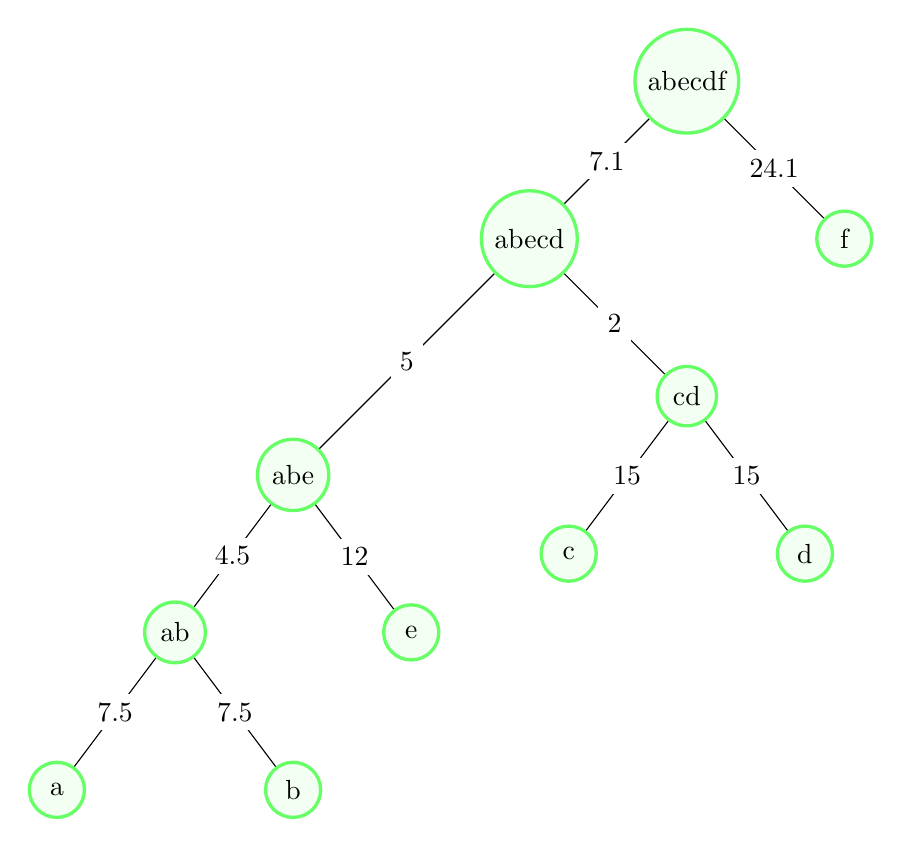
\begin{tikzpicture}[roundnode/.style={circle, draw=green!60, fill=green!5, very thick, minimum size=7mm}]
		\node[roundnode]	(a) at (-3,-5)	{a};
		\node[roundnode]	(b) at (0,-5)	{b};
		\node[roundnode]	(ab) at (-1.5,-3)	{ab};
		\node[roundnode]	(e) at (1.5,-3)	{e};
		\node[roundnode]	(abe) at (0,-1)	{abe};
		\node[roundnode]	(c) at (3.5,-2)	{c};
		\node[roundnode]	(d) at (6.5,-2)	{d};
		\node[roundnode]	(cd) at (5,0)	{cd};
		\node[roundnode]	(abecd) at (3,2)	{abecd};
		\node[roundnode]	(f) at (7,2)	{f};
		\node[roundnode]	(abecdf) at (5,4)	{abecdf};
		
		\draw[-] (a) -- (ab) node [midway, fill=white] {7.5};
		\draw[-] (b) -- (ab) node [midway, fill=white] {7.5};
		\draw[-] (ab) -- (abe) node [midway, fill=white] {4.5};
		\draw[-] (e) -- (abe) node [midway, fill=white] {12};
		\draw[-] (c) -- (cd) node [midway, fill=white] {15};
		\draw[-] (d) -- (cd) node [midway, fill=white] {15};
		\draw[-] (abe) -- (abecd) node [midway, fill=white] {5};
		\draw[-] (cd) -- (abecd) node [midway, fill=white] {2};
		\draw[-] (abecd) -- (abecdf) node [midway, fill=white] {7.1};
		\draw[-] (f) -- (abecdf) node [midway, fill=white] {24.1};
		
		\end{tikzpicture}
	\end{center}
\end{document}